\documentclass[tikz]{standalone}

\usetikzlibrary{calc,positioning}

% Create fake \onslide and other commands for standalone picture
\usepackage{xparse}
\NewDocumentCommand{\onslide}{s t+ d<>}{}
\NewDocumentCommand{\only}{d<>}{}
\NewDocumentCommand{\uncover}{d<>}{}
\NewDocumentCommand{\visible}{d<>}{}
\NewDocumentCommand{\invisible}{d<>}{}

\begin{document}

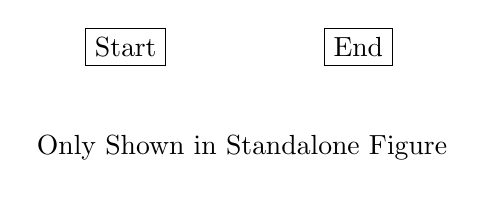
\begin{tikzpicture}
  \node[draw] (start) { Start };
  \node[draw, right=2cm of start] (end) { End };
  % The following animation will only have affect in beamer.
  % In standalone mode, the figure is static.
%  \onslide<2-> { \draw[-latex] (start) -- (end); }
  \coordinate (mid) at ($(start)!.5!(end)$);

  % We could control parts of figure only shown in beamer or vice versa.
  \ifstandalone
    \node[below=1cm of mid] {Only Shown in Standalone Figure};
  \else
    \node[below=1cm of mid] {Only Shown in Beamer};
  \fi
\end{tikzpicture}

\end{document}